\chapter{Loss function}

The objective function is composed by the data loss and a regularization term. The data loss takes the form of an average over the data losses for every individual example. That is, $L = \frac{1}{N} \sum_i L_i$ where $N$ is the number of training data. Lets abbreviate $f = f(x_i; W)$ to be the activations of the output layer in a Neural Network. There are several types of problems you might want to solve in practice:

\section*{Classification}

We assume a dataset of examples and a single correct label (out of a fixed set) for each example. One of two most commonly seen cost functions in this setting are the \textit{SVM} (e.g. the Weston Watkins formulation):

\begin{equation}
L_i = \sum_{j\neq y_i} \max(0, f_j - f_{y_i} + 1)
\end{equation}

where $f_{y_i}$ is the activation of the correct class, and $f_{j}$ the activation of the class $j$. As we briefly alluded to, some people report better performance with the squared hinge loss (i.e. instead using $\max(0, f_j - f_{y_i} + 1)^2$). The second common choice is the \textit{Softmax classifier} that uses the cross-entropy loss. It transforms the \textit{logits} (scores) output of the network and transforms them into probabilities.

\begin{equation}
L_i = -\log\left(\frac{e^{f_{y_i}}}{ \sum_j e^{f_j} }\right)
\end{equation}

In some rough sense, the cross-entropy is measuring how inefficient our predictions are for describing the truth. 

Probabilistic interpretation. Looking at the expression, we see that

\begin{equation}
P(y_i \mid x_i;W) = \frac{e^{f_{y_i}}}{ \sum_j e^{f_j} }
\end{equation}

can be interpreted as the (normalized) probability assigned to the correct label $y_i$ given the image $x_i$ and parameterized by $W$. To see this, remember that the Softmax classifier interprets the scores inside the output vector $f$ as the unnormalized log probabilities (log probabilities means representing probabilities in logarithmic space, instead of the standard [0,1] interval. This has practical advantages because computers can perform addition more efficiently than multiplication). Exponentiating these quantities therefore gives the (unnormalized) probabilities, and the division performs the normalization so that the probabilities sum to one. In the probabilistic interpretation, we are therefore minimizing the negative log likelihood of the correct class, which can be interpreted as performing \textit{Maximum Likelihood Estimation} (MLE). A nice feature of this view is that we can now also interpret the regularization term $R(W)$ in the full loss function as coming from a Gaussian prior over the weight matrix $W$, where instead of MLE we are performing the \textit{Maximum a posteriori} (MAP) estimation. We mention these interpretations to help your intuitions, but the full details of this derivation are beyond the scope of this class.

\begin{figure}[h]
  \centering
  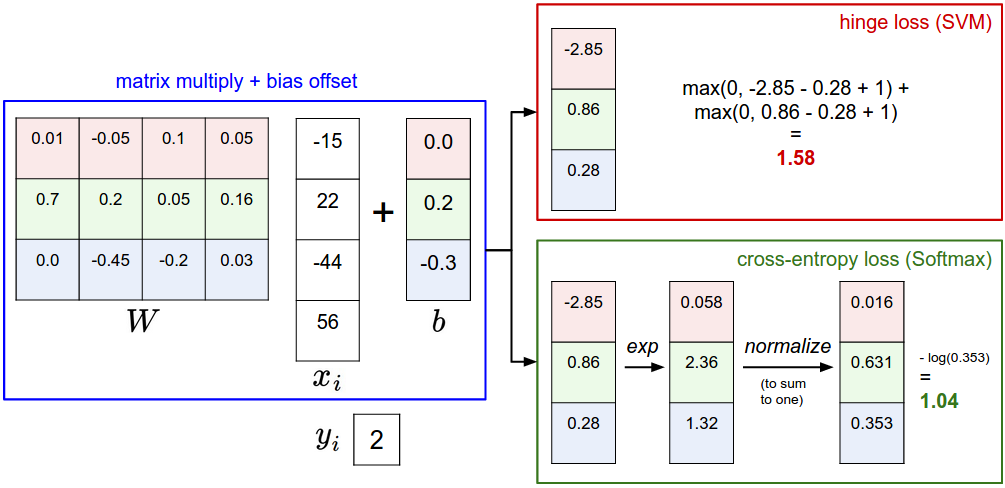
\includegraphics[width=0.8\textwidth]{Images/loss_f/1.png}
  \caption{Example of the difference between the SVM and Softmax classifiers for one datapoint. In both cases we compute the same score vector f (e.g. by matrix multiplication in this section). The difference is in the interpretation of the scores in f: The SVM interprets these as class scores and its loss function encourages the correct class (class 2, in blue) to have a score higher by a margin than the other class scores. The Softmax classifier instead interprets the scores as (unnormalized) log probabilities for each class and then encourages the (normalized) log probability of the correct class to be high (equivalently the negative of it to be low). The final loss for this example is 1.58 for the SVM and 1.04 (note this is 1.04 using the natural logarithm, not base 2 or base 10) for the Softmax classifier, but note that these numbers are not comparable; They are only meaningful in relation to loss computed within the same classifier and with the same data.}
\end{figure}

\subsection*{Problem}

Large number of classes. When the set of labels is very large (e.g. words in English dictionary, or ImageNet which contains 22,000 categories), it may be helpful to use \textit{Hierarchical Softmax}. The hierarchical softmax decomposes labels into a tree. Each label is then represented as a path along the tree, and a Softmax classifier is trained at every node of the tree to disambiguate between the left and right branch. The structure of the tree strongly impacts the performance and is generally problem-dependent.

\section*{Attribute Classification}
Both losses above assume that there is a single correct answer $y_i$. But what if $y_i$ is a binary vector where every example may or may not have a certain attribute, and where the attributes are not exclusive? For example, images on Instagram can be thought of as labeled with a certain subset of hashtags from a large set of all hashtags, and an image may contain multiple. A sensible approach in this case is to build a binary classifier for every single attribute independently. For example, a binary classifier for each category independently would take the form:

\begin{equation}
L_i = \sum_j \max(0, 1 - y_{ij} f_j)
\end{equation}

where the sum is over all categories $j$, and $y_{ij}$ is either +1 or -1 depending on whether the i-th example is labeled with the j-th attribute, and the score vector $f_j$ will be positive when the class is predicted to be present and negative otherwise. Notice that loss is accumulated if a positive example has score less than +1, or when a negative example has score greater than -1.

An alternative to this loss would be to train a logistic regression classifier for every attribute independently. A binary logistic regression classifier has only two classes (0,1), and calculates the probability of class 1 as:

\begin{equation}
P(y = 1 \mid x; w, b) = \frac{1}{1 + e^{-(w^Tx +b)}} = \sigma (w^Tx + b)
\end{equation}

Since the probabilities of class 1 and 0 sum to one, the probability for class 0 is $P(y = 0 \mid x; w, b) = 1 - P(y = 1 \mid x; w,b)$. Hence, an example is classified as a positive example (y = 1) if $\sigma (w^Tx + b) > 0.5$, or equivalently if the score $w^Tx +b > 0$. The loss function then maximizes the log likelihood of this probability. You can convince yourself that this simplifies to:

\begin{equation}
L_i = \sum_j y_{ij} \log(\sigma(f_j)) + (1 - y_{ij}) \log(1 - \sigma(f_j))
\end{equation}

where the labels $y_{ij}$ are assumed to be either 1 (positive) or 0 (negative), and $\sigma(\cdot)$ is the sigmoid function. The expression above can look scary but the gradient on $f$ is in fact extremely simple and intuitive: $\partial{L_i} / \partial{f_j} = y_{ij} - \sigma(f_j)$ (as you can double check yourself by taking the derivatives).

\section*{Regression}
Regression is the task of predicting real-valued quantities, such as the price of houses or the length of something in an image. For this task, it is common to compute the loss between the predicted quantity and the true answer and then measure the L2 squared norm, or L1 norm of the difference. The L2 norm squared would compute the loss for a single example of the form:

\begin{equation}
L_i = \Vert f - y_i \Vert_2^2
\end{equation}

The reason the L2 norm is squared in the objective is that the gradient becomes much simpler, without changing the optimal parameters since squaring is a monotonic operation. The L1 norm would be formulated by summing the absolute value along each dimension:

\begin{equation}
L_i = \Vert f - y_i \Vert_1 = \sum_j \mid f_j - (y_i)_j \mid
\end{equation}

where the sum $\sum_j$ is a sum over all dimensions of the desired prediction, if there is more than one quantity being predicted. Looking at only the j-th dimension of the i-th example and denoting the difference between the true and the predicted value by $\delta_{ij}$, the gradient for this dimension (i.e. $\partial{L_i} / \partial{f_j}$ is easily derived to be either $\delta_{ij}$ with the L2 norm, or $sign(\delta_{ij})$. That is, the gradient on the score will either be directly proportional to the difference in the error, or it will be fixed and only inherit the sign of the difference.

\paragraph*{Outliers} L2 norm is not that good dealing with outliers in the training samples. You may consider L1 or variations of L2.

\paragraph*{Word of caution} It is important to note that the L2 loss is much harder to optimize than a more stable loss such as Softmax. Intuitively, it requires a very fragile and specific property from the network to output exactly one correct value for each input (and its augmentations). Notice that this is not the case with Softmax, where the precise value of each score is less important: It only matters that their magnitudes are appropriate. Additionally, the L2 loss is less robust because outliers can introduce huge gradients. When faced with a regression problem, first consider if it is absolutely inadequate to quantize the output into bins. For example, if you are predicting star rating for a product, it might work much better to use 5 independent classifiers for ratings of 1-5 stars instead of a regression loss. Classification has the additional benefit that it can give you a distribution over the regression outputs, not just a single output with no indication of its confidence. If you’re certain that classification is not appropriate, use the L2 but be careful: For example, the L2 is more fragile and applying dropout in the network (especially in the layer right before the L2 loss) is not a great idea.

When faced with a regression task, first consider if it is absolutely necessary. Instead, have a strong preference to discretizing your outputs to bins and perform classification over them whenever possible.

\section*{Structured prediction}
The structured loss refers to a case where the labels can be arbitrary structures such as graphs, trees, or other complex objects. Usually it is also assumed that the space of structures is very large and not easily enumerable. The basic idea behind the structured SVM loss is to demand a margin between the correct structure $yi$ and the highest-scoring incorrect structure. It is not common to solve this problem as a simple unconstrained optimization problem with gradient descent. Instead, special solvers are usually devised so that the specific simplifying assumptions of the structure space can be taken advantage of. We mention the problem briefly but consider the specifics to be outside of the scope of the class.